\documentclass{article}
\usepackage{amsmath}
\usepackage{amssymb}
\usepackage{graphicx}
\usepackage{hyperref}
\usepackage[version=4]{mhchem}

\title{Problem 6}
\date{}

\begin{document}
\maketitle

\section*{Problem}
In \(\triangle A B C, \angle B=2 \angle A\) and \(A B=2 B C\). Show that \(A B^{2}=A C^{2}+B C^{2}\).\\
\centering
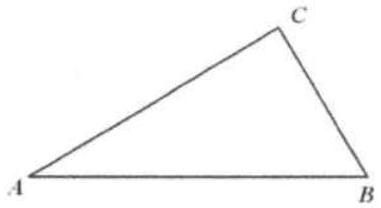
\includegraphics[width=\textwidth]{images/problem_image_1.jpg}

\section*{Solution}
Since \(A B>B C, \angle C>\angle A\).\\
Draw \(C D\) to meet \(A B\) at \(D\) such that \(\angle A C D=\angle A\).\\
\(\triangle A D C\) is an isosceles triangle and \(A D=D C\).\\
\(\angle C D B=\angle A C D+\angle A=2 \angle A=\angle B\)\\
\centering
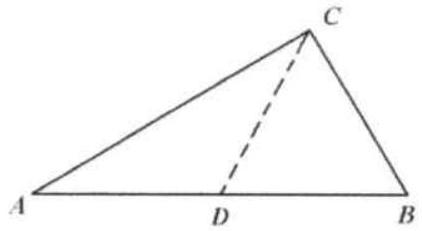
\includegraphics[width=\textwidth]{images/reasoning_image_1.jpg}

Therefore, \(\triangle B C D\) is also an isosceles triangle, and so \(D C=B C\).\\
\(A B=A D+D B=2 B C\)\\
\(\Rightarrow \quad A D+D B=2 D C=2 A D\)\\
\(\Rightarrow \quad A D=D B=D C\).

This tells us that \(D C\) is the median of right triangle \(A B C\) with \(\angle C=90^{\circ}\).\\
By the Pythagorean Theorem, we have \(A B^{2}=A C^{2}+B C^{2}\).

\end{document}
